
\section{B2}
\subsection{B2.1ddf}
\subsection{B2.2}

First, the formula is converted into existential normal form:

$\neg (EX \Phi_1) \wedge (\neg (EG \neg \Phi_2))$

The abstract syntax tree consists purely of state formula,
with the path operators included with their enclosing path quantifier:

\begin{figure}[!htb]
\centering
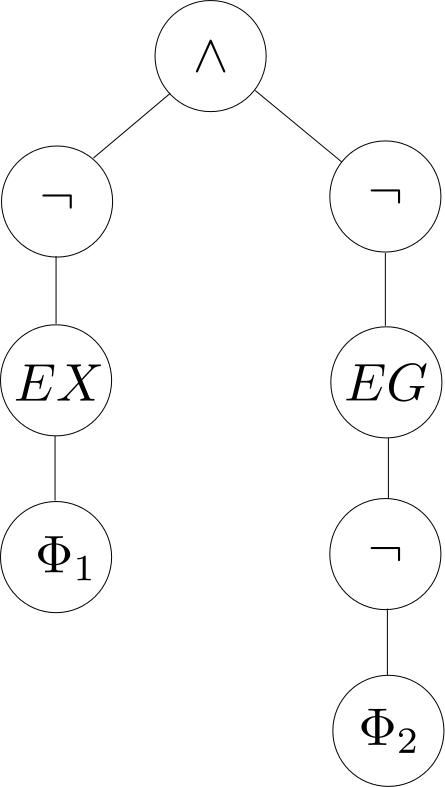
\includegraphics[scale=.4]{abstract_syntax_tree.png}
\caption{Abstract syntax tree}
\label{fig:ast}
\end{figure}

The sub-terms are defined from the atoms up:

$\Phi_1: Sat(\Phi_1)$

$EX \Phi_1: \{s \in S | Succ(s) \cap Sat(\Phi_1) \neq \emptyset\}$

$\neg (EX \Phi_1): S \setminus \{s \in S | Succ(s) \cap Sat(\Phi_1) \neq \emptyset\}$

$\Phi_2: Sat(\Phi_2)$

$\neg \Phi_2: S \setminus Sat(\Phi_2)$

$EG \neg \Phi_2: T, \text{    where } \{s \in S \setminus Sat(\Phi_2) | Succ(s) \cap T \neq \emptyset \} \supseteq T, \text{greatest } T$

$\neg (EG \neg \Phi_2): S \setminus Sat(EG \neg \Phi_2)$

$\neg (EX \Phi_1) \wedge (\neg (EG \neg \Phi_2)): Sat(\neg (EX \Phi_1)) \cap Sat(\neg (EG \neg \Phi_2))$

A sub-term whose set of states is defined recursively is the sub-term $EG \neg \Phi_2$.
The recursion equation is $\{s \in S \setminus Sat(\Phi_2) | Succ(s) \cap T \neq \emptyset \} \supseteq T$.
This equation has many solutions.
Replacing the subset operator with equal, the recursion equation can be seen as a function $f$ of $T$.
The only solutions are then fixed-points of $f$.
A fixed-point for $f$ is a value $x_0$ that makes the following equation true: $x_0 = f(x_0)$,
namely, applying the function to the value gives the value itself, "fixed" in some sense.
It can be shown that the solutions have a unique least solution and a unique greatest solution,
or since the solutions is the same as the fixed-points for the function, a least fixed-point and a greatest fixed-point.
The least fixed-point is the empty set.
The greatest fixed-point is more interesting, and is exactly equal to $EG \neg \Phi_2$.
If the equation had not been an existential-always, but an existential-until or
an existential-eventually, the interesting fixed point would be the least fixed point.

The solution to the transition system $M_1$ can be calculated recursively,
using the sets found for each sub-term:

$\Phi_1: Sat(\Phi_1): \{s_0, s_4, s_5\}$

$EX \Phi_1: \{s \in S | Succ(s) \cap Sat(\Phi_1) \neq \emptyset\}: \{s_1, s_2, s_3\}$

$\neg (EX \Phi_1): S \setminus Sat(EX \Phi_1): \{s_0, s_4, s_5\}$

$\Phi_2: Sat(\Phi_2): \{s_1, s_2, s_3\}$

$EG \neg \Phi_2: \neg \Phi_2: S \setminus Sat(\Phi_2): \{s_0, s_4, s_5\}$

$EG \neg \Phi_2: T, \text{    where } \{s \in Sat(\neg \Phi_2) | Succ(s) \cap T \neq \emptyset \} \supseteq T, \text{greatest } T: \{\}$

$\neg (EG \neg \Phi_2): S \setminus Sat(EG \neg \Phi_2): \{s_0, s_1, s_2, s_3, s_4, s_5\}$

$\neg (EX \Phi_1) \wedge (\neg (EG \neg \Phi_2)): Sat(\neg (EX \Phi_1)) \cap Sat(\neg (EG \neg \Phi_2)): \{s_0, s_4, s_5\}$

